%%%%%%%%%%%%%%%%%%%%%%%%%%%%%%%%%%%%%%%%%
% The Commander X16 User's Manual
%
% Authors:
% Jestin Stoffel (jestin.stoffel@gmail.com)
%
% License:
% CC BY-NC-SA 4.0 (https://creativecommons.org/licenses/by-nc-sa/4.0/)
%
% Compiling this template:
% This template uses biber for its bibliography and makeindex for its index.
% When you first open the template, compile it from the command line with the 
% commands below to make sure your LaTeX distribution is configured correctly:
%
% 1) pdflatex main
% 2) makeindex main.idx -s indexstyle.ist
% 3) biber main
% 4) pdflatex main x 2
%
% After this, when you wish to update the bibliography/index use the appropriate
% command above and make sure to compile with pdflatex several times 
% afterwards to propagate your changes to the document.
%
%%%%%%%%%%%%%%%%%%%%%%%%%%%%%%%%%%%%%%%%%

%----------------------------------------------------------------------------------------
%	PACKAGES AND OTHER DOCUMENT CONFIGURATIONS
%----------------------------------------------------------------------------------------

\documentclass[
	11pt, % Default font size, select one of 10pt, 11pt or 12pt
	fleqn, % Left align equations
	letterpaper, % Paper size, use either 'a4paper' for A4 size or 'letterpaper' for US letter size
	%oneside, % Uncomment for oneside mode, this doesn't start new chapters and parts on odd pages (adding an empty page if required), this mode is more suitable if the book is to be read on a screen instead of printed
]{CommodoreBlueBook}

% Book information for PDF metadata, remove/comment this block if not required 
\hypersetup{
	pdftitle={Title}, % Title field
	pdfauthor={Author}, % Author field
	pdfsubject={Subject}, % Subject field
	pdfkeywords={Keyword1, Keyword2, ...}, % Keywords
	pdfcreator={LaTeX}, % Content creator field
}

\addbibresource{sample.bib} % Bibliography file

\definecolor{blue}{rgb}{0.0,0.0,0.8}
\definecolor{gray}{rgb}{0.73, 0.73, 0.73}

%----------------------------------------------------------------------------------------

\begin{document}

%----------------------------------------------------------------------------------------
%	COVER PAGE
%----------------------------------------------------------------------------------------

\coverpage % Output the title page
	{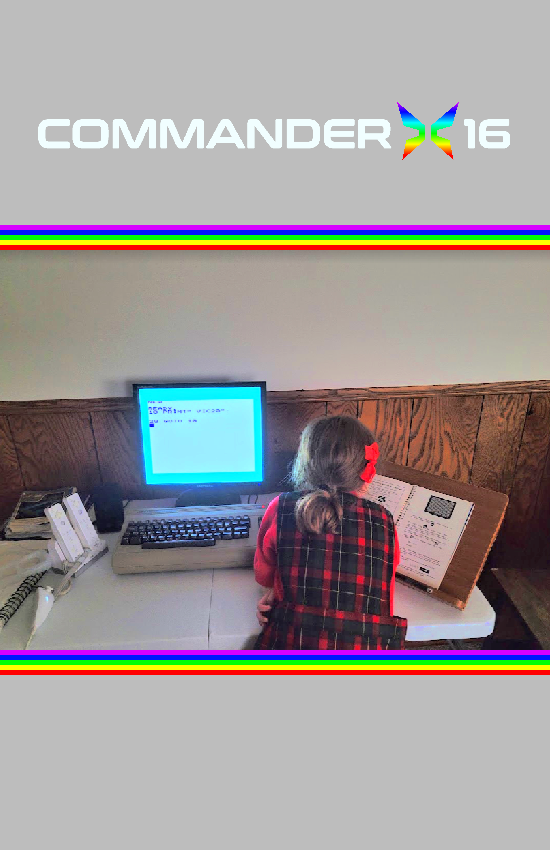
\includegraphics[width=\paperwidth]{cover.png}} % Code to output the background image, which should be the same dimensions as the paper to fill the page entirely; leave empty for no background image
	{ % Title(s) and author(s)
		\centering\rmfamily % Font styling
		{\Huge\bfseries Retro Computing on the\par} % Top
	}
	{
		\centering\rmfamily % Font styling
		{\huge\bfseries a friendly computer guide\par} % Bottom
	}

%----------------------------------------------------------------------------------------
%	COPYRIGHT PAGE
%----------------------------------------------------------------------------------------

\thispagestyle{empty} % Suppress headers and footers on this page

~\vfill % Push the text down to the bottom of the page

% \noindent \textsc{Published by Publisher}\\ % Publisher

\noindent \textsc{\href{https://www.commanderx16.com}{commanderx16.com}}\\ % URL

\noindent \textit{1st Edition}\\ % Printing/edition date

\noindent Copyright \copyright\ 2022 Jestin Stoffel\\ % Copyright notice

\noindent Licensed under the Creative Commons Attribution-NonCommercial 4.0
License (the ``License''). You may not use this file except in compliance with
the License. You may obtain a copy of the License at
\url{https://creativecommons.org/licenses/by-nc-sa/4.0}. Unless required by
applicable law or agreed to in writing, software distributed under the License
is distributed on an \textsc{``as is'' basis, without warranties or conditions
of any kind}, either express or implied. See the License for the specific
language governing permissions and limitations under the License.\\ % License information, replace this with your own license (if any)

\cleardoublepage % Start the following content on a new page
\pagenumbering{Roman}

%----------------------------------------------------------------------------------------
%	TITLE PAGE
%----------------------------------------------------------------------------------------
\pagecolor{blue}

\afterpage{
	\thispagestyle{part} % use part header/footer style
	\newgeometry{
		top=1.5in, % Top margin
		bottom=0.5cm, % Bottom margin
		right=0.75in, % Right margin
		}
	\begin{flushright}
		{
			\huge\sffamily\bfseries\color{white}
			RETRO\\ COMPUTING\\ ON THE\\
			\vspace{8pt}
			{
				\contourlength{2pt}
				\contournumber{20}
				\fontsize{36pt}{36pt}\selectfont Commander
				\contour{white}{\textcolor{blue} {X16}}
			}
		}
		\huge\sffamily\color{white} A friendly computer guide
	\end{flushright}
	\clearpage
	\restoregeometry
}

\clearpage

\nopagecolor % Change page color back

%----------------------------------------------------------------------------------------
%	PREFACE PAGE
%----------------------------------------------------------------------------------------

\section*{PREFACE}
\addcontentsline{toc}{chapter}{\protect\numberline{}PREFACE}

\par You are about to meet a computer that feels out of place for its time.  It
is slower, larger, and more expensive than most computers of its era.  In many
ways, it is a technological anachronism designed for a niche market of
hobbyists and enthusiasts.  But that's not all.

\medskip
\par The Commander X16 reaches into the past and brings back many things that
were lost.  It is a computer that recaptures the "soul" of the early days of
home computing.  Together with this manual, anyone should be able to sit down
and begin to explore computing with all the modern layers of abstraction
stripped away.  No prior knowledge of computing or even typing should be
required in order to start your journey into the world of computers!

\medskip
\par This manual should be readable by experts and novices alike.  Even children as
young as 6 or 7 should be able to follow along with the step-by-step examples.
There is no reason you need to read this manual in order.  After reading
Chapter 1 (Getting Started) you can go directly to a chapter that interests you
and start reading.  The first page of each chapter contains a small sample
program to type in.  Type it exactly for a demonstration of what you will learn
in that chapter.  The rest of the chapter will explain the details as you read,
and contain more sample programs to try out.

% \medskip
% \par The Commander X16 was created with the intention that you can simply turn it on
% and start learning, doing, and creating.  The friendly blue screen and colorful
% butterfly logo invite you to start typing BASIC commands and programs.  The
% built-in SD card reader allows you to save your work as well as load the
% programs and art that others create, all without needing to troubleshoot
% expensive antique disk drives and data sets...although it supports those too!

\medskip
\par Computers have become an important part of our everyday lives, and yet most
people never delve past the surface of the user interfaces presented to them.
Children are given touch screen devices before they can even talk, and adults
go through their entire lives without learning about the magic that happens
behind their screens.  The Commander X16 reverses this trend by putting the
user back in control of a computer that they can fully understand.

\medskip
\par The Commander X16 is the perfect computer for this day and age!


\cleardoublepage % Start the following content on a new page

%----------------------------------------------------------------------------------------
%	TABLE OF CONTENTS
%----------------------------------------------------------------------------------------

\pagestyle{empty} % Disable headers and footers for the following pages

\setcounter{tocdepth}{0}
\tableofcontents % Output the table of contents

% \listoffigures % Output the list of figures, comment or remove this command if not required
% 
% \listoftables % Output the list of tables, comment or remove this command if not required

\pagestyle{fancy} % Enable default headers and footers again

\clearpage % Start the following content on a new page

%----------------------------------------------------------------------------------------
%	SETUP PAGE
%----------------------------------------------------------------------------------------

\section*{SETUP}
\addcontentsline{toc}{section}{\protect\numberline{}SETUP}

Autem eos placeat est in iure. Qui tempora ut ut qui dolores unde. Nesciunt
omnis cum iusto laboriosam ut. Amet similique omnis sit maxime laudantium.
Nobis delectus ut corrupti et excepturi. Aut amet error cumque eaque explicabo
quo unde. Minus consectetur error atque ut. Alias ut repudiandae eum eum.
Quaerat rerum facilis suscipit dolores qui consequatur aut perferendis. Et
alias est autem fugit enim nobis qui illo. Error nesciunt et adipisci ex
nostrum. Laudantium sit et ut est voluptatum dolor. Ea vitae soluta consectetur
vel culpa reiciendis. Ad est officiis ut consectetur sint voluptatem aut dolor.
Tempora consequuntur suscipit asperiores exercitationem. Harum officia nisi
omnis ut iste rerum. Consequatur tempora maxime ipsa velit sit. Consequatur
ipsum necessitatibus autem ut saepe eum quod ea. Omnis qui non et minima
perferendis sunt repudiandae. Voluptas minima earum est libero inventore
corporis est sint. Occaecati odio distinctio est. Ab quidem asperiores deleniti
soluta debitis exercitationem veniam. Ut sit quo accusantium velit quam
voluptatum quia quia. Non sed non consequatur corrupti sed libero. Vitae
dolores id distinctio enim magni sed omnis.

Voluptates ipsa animi et a iusto. Qui doloribus ducimus voluptas sunt quidem
similique animi blanditiis. Cupiditate dolorum quia illo. Totam sit consequatur
quos. Ipsa dolorum dolor dolores ad deserunt eum debitis. Id quae porro
eligendi tempora magni qui odit. Recusandae et placeat officia blanditiis
perspiciatis quaerat. At saepe perspiciatis explicabo. Non sit quam
exercitationem sequi commodi tempore et quasi. Tempora distinctio et voluptatum
reiciendis qui minus deleniti. Quidem officiis eveniet debitis voluptas sint
provident numquam architecto. Eligendi quibusdam rerum debitis possimus et
ratione enim quasi. Placeat minus beatae sed aut est. Itaque quisquam eum
adipisci enim rerum qui. Dolor at veniam est molestiae. Sed velit sunt est
consequatur suscipit. Quisquam et ipsum qui est et accusantium porro omnis.
Asperiores enim eos eos. Unde officiis quo est ex expedita odit. Vel maiores
animi non dolor molestiae quia rerum aut. Vel tempore non doloremque sint
nesciunt. Ipsa voluptas qui repellat id earum temporibus ut soluta. Pariatur
esse beatae autem et consequatur repellendus cum dolores. A aliquam porro
voluptatem repellat dolorem. Doloribus voluptas aspernatur in veniam est iusto.

Eveniet dolorum maiores vitae. Rerum culpa et consequatur. Cumque tenetur
dolorem autem voluptatum. Omnis aut nihil odio ipsam et. Fugiat fuga molestias
earum ut neque odit. Cumque odio sapiente qui aliquid. Veritatis quasi
voluptates quis illo accusantium. Dolorum vitae sunt et quis eos incidunt vel
iusto. Aliquam eos eaque aut qui placeat ut modi. Modi ipsa quas dolor qui nam.
Deserunt magnam officiis sunt harum aspernatur rem voluptas tempore.
Consequuntur consequatur in vel velit architecto quo cumque. Ea aspernatur
pariatur velit eveniet quibusdam atque officiis. Quidem tempore quia
consectetur autem alias necessitatibus rerum. Accusantium similique odio ut
consectetur qui est. Quia modi laudantium minima et cumque et qui. Doloribus
magni quia cum totam porro. Voluptas corporis ea blanditiis possimus omnis
maiores. Quo autem esse eligendi occaecati eos nihil. Quae eius inventore
recusandae molestiae qui autem veniam. Doloribus quos deleniti consequatur
saepe saepe rerum maxime aliquam. Ut sed ipsam dolorum maxime laboriosam hic
quibusdam est. Et consequatur aut provident numquam aut quisquam. Officia nulla
atque aut illum rerum deserunt dolor maxime. Ea libero est doloremque odio.



\cleardoublepage

\pagenumbering{arabic} % Reset page numbers and use arabic

%----------------------------------------------------------------------------------------
%	PART - Getting to Know Your Commander X16
%----------------------------------------------------------------------------------------

%----------------------------------------------------------------------------------------
%	PART - Getting to Know Your Commander X16
%----------------------------------------------------------------------------------------

\makeatletter\@openrightfalse
\part{Getting to Know Your Commander X16}

\chaptertypein{
	\keybackgroundcolor{gray}
	\keytextcolor{black}
	1 PRINT "X16" \returnkey\\\\
	2 GOTO 1 \returnkey\\
}

\begin{tikzpicture}
	\hyphenpenalty=10000
	\bubble{2.5in}{2.5in}{4.8}{6.3}{
		This line tells the X16 to print what's between the quotation marks.}
	\bubble{2.5in}{1.75in}{4.0}{5.2}{
		This line tells the X16 to go back to Line 1 and print it again.}
	\bubble{2.5in}{1.1in}{6.0}{2.0}{
		Typing the word RUN makes the program run.}
\end{tikzpicture}

%----------------------------------------------------------------------------------------
%	CHAPTER - Getting Started
%----------------------------------------------------------------------------------------

\chapter*{Getting Started}\index{Sectioning}
\addcontentsline{toc}{chapter}{\protect\numberline{}Getting Started}


Congratulations!  Your Commander X16 is up and running and ready to accept your
first commands.  When it starts, it should display a message at the top letting
you know that it is running BASIC and how much memory is available.  There will
also be a white blinking rectangle called a \emph{cursor}.  This is how the X16
signals that it is waiting for you.

\section{The Start Screen}

\screenbox{2.75in}{2in}{
	**** X16 BASIC ****\\
	512k HIGH RAM\\
	38655 BASIC BYTES FREE\\\\
	READY.\\
	\cursor
}

\begin{tikzpicture}
	\hyphenpenalty=10000
	\tinybubble{3.0in}{1.2in}{1.0}{3.05}{
		The X16 is saying it's ready.
		}
\end{tikzpicture}

\vspace{16pt}

\tip{deleting characters}{
	\keybackgroundcolor{gray}
	\keytextcolor{black}

	If you type a character on the screen that you don't want, press the
	\backspacekey key.  This key will erase the character immediately to the
	left of the cursor.\\

	Use this key as often as you like to delete unwanted characters.
}

\section{A Quick Experiement}

\keybackgroundcolor{white}
\keytextcolor{black}

It's time to start pressing keys and giving your Commander X16 something to do!
Press the following keys:\\

\key{p} \key{r} \key{i} \key{n} \key{t}\\



As you press each key, the cursor moves to the right.  The cursor will always
show you where the next character will be typed.  Next, locate one of the
\shiftkey keys on the keyboard.  There will be one on the right and one on the
left, but they both do the same thing: modify another key when pressed at the
same time as \shiftkey.\\

Hold down the \shiftkey key and press the
\keybackgroundcolor{white}\doublekey{"\\'} key.  The screen should now look
like this:\\

\screenbox{2.75in}{2in}{
	**** X16 BASIC ****\\
	512k HIGH RAM\\
	38655 BASIC BYTES FREE\\\\
	READY.\\
	PRINT"\cursor
}

\begin{tikzpicture}
	\hyphenpenalty=10000
	\smallbubble{3.0in}{1.0in}{2.2}{2.8}{
		You typed this.
		}
\end{tikzpicture}

Pressing the \doublekey{"\\'} key while holding down \shiftkey caused the
{\ttfamily "} character to by typed instead of the {\ttfamily '} character.\\

Now let't type a word.  Without holding down any other keys, press these keys:\\

\keybackgroundcolor{white}
\key{b} \key{u} \key{t} \key{t} \key{e} \key{r} \key {f} \key{l} \key{y}\\

Finally, hold down the \shiftkey key, and press the
\keybackgroundcolor{white}\doublekey{"\\'} key one more time.  The screen
should now show:\\

{
	\raggedleft
	\screenbox{2.75in}{2in}{
		**** X16 BASIC ****\\
		512k HIGH RAM\\
		38655 BASIC BYTES FREE\\\\
		READY.\\
		PRINT"BUTTERFLY"\cursor
	}
}

\begin{tikzpicture}
	\hyphenpenalty=10000
	\smallbubble{0in}{1.1in}{4.8}{2.8}{
		Everything you typed is on this line.}
\end{tikzpicture}

If something doesn't look correct, use the \backspacekey key to delete
characters and then you can re-type them.\\

Once everything looks correct, find the \returnkey key on the keyboard
and press it once.  Now look at your screen.

\screenbox{3.5in}{2.625in}{
	**** X16 BASIC ****\\
	512k HIGH RAM\\
	38655 BASIC BYTES FREE\\\\
	READY.\\
	PRINT"BUTTERFLY"\\
	BUTTERFLY\\\\
	READY.\\
	\cursor
}

\begin{tikzpicture}
	\hyphenpenalty=10000
	\smallbubble{2.5in}{2.3in}{3.8}{4.8}{You typed this.}
	\bubble{2.5in}{1.8in}{4.2}{4.4}{
		The cursor was here when you pressed the \returnkey key.}
	% because I need 3 arrows, I just print this 3 times with different
	% settings.  The final bubble will be drawn over the others.
	\bubble{2.5in}{1.2in}{2.9}{3.9}{
		The Commander X16 printed these.}
	\bubble{2.5in}{1.2in}{2.0}{3.0}{
		The Commander X16 printed these.}
	\bubble{2.5in}{1.2in}{1.0}{2.5}{
		The Commander X16 printed these.}
\end{tikzpicture}

Pressing the \returnkey key told the X16 that you were finished typing your
command.  Then the X16 looked at the command you typed, saw that it was
something it knows how to do, and then did it.  In this case, your command told
the X16 to {\ttfamily PRINT} a message to the screen,  The X16 knew \emph{what}
to print because you told it that as well by placing your message between the
quotation marks.\\

When the X16 finished {\ttfamily PRINT}ing the word {\ttfamily BUTTERFLY}, it
let you know by displaying the {\ttfamily READY} message and blinking the
cursor.\\

\note{

	If you are not using an official Commander X16 keyboard, then you probably
	won't have a \returnkey key, but instead have an \returnkey key.  Don't
	worry, they are the same thing.

}

\section{Your Own Experiments}

Now that you've {\ttfamily PRINT}ed something to the screen, try {\ttfamily
PRINT}ing other things.  Can you make the Commander X16 say {\ttfamily HELLO}?
Can you make it say your name?\\

Here are some things to keep in mind:

\begin{itemize}
	\item Make sure you spell the word {\ttfamily PRINT} correctly
	\item Put your message between quotation marks ({\ttfamily "}).  Make sure
		you have one quotation mark at the beginning and one at the end
	\item Run your command by pressing \returnkey
	\item If something isn't working as you expect, continuing reading to learn about errors
\end{itemize}

\section{Making A Mistake On Purpose}

What happens if you type something wrong?  Anyone who spends any amount of time
using a computer is going to mistype a command.  Let's find out what happens by
making a mistake \emph{on purpose}.  That way, we understand what is happening
when we make a mistake \emph{by accident}.  Let's make a mistake!\\

Try typing our first command, but this time misspell {\ttfamily PRINT} by
forgetting the {\ttfamily I} and typing {\ttfamily PRNT} instead:

\screenbox{2.75in}{2in}{
	READY.\\
	PRNT"BUTTERFLY"\cursor
}

This is a very easy mistake to make, and at a glace you won't even notice that
the command is wrong.  Now press \returnkey to run this command.  You should
see an error message:

{
	\raggedleft
	\screenbox{2.75in}{2in}{
		READY.\\
		PRNT"BUTTERFLY"\\\\
		?SYNTAX ERROR\\
		READY.\\
		\cursor
	}
}

\begin{tikzpicture}
	\hyphenpenalty=10000
	\smallbubble{0in}{1.5in}{4.9}{3.7}{The X16 lets you know that something is wrong.}
\end{tikzpicture}

Printing {\ttfamily ?SYNTAX ERROR} to the screen is how the X16 tells you that
you typed something that it does not understand.  In this case, you typed
{\ttfamily PRNT} instead of {\ttfamily PRINT}.\\

For now, don't worry about these errors.  Just do you best to you type your
commands correctly before you press \returnkey.

As you experiment with typing commands, the screen will scroll down to give you
more room to type and more room for the Commander X16 to print the results of
your commands.  You may want to clear the screen and bring the cursor back to
the top.  The Commander X16 has a built-in way to do this without even typing a
command:\\

Hold down the \shiftkey key and press the \clrhomekey key.\\

This clears the screen immediately and places the cursor at the top of the
screen.\\

\tip{Clearing The Screen}{

	Clearing the screen will be one of the most frequent things you do while
	working on your Commander X16.  It is worth memorizing the \shiftkey
	\clrhomekey key combination so that you don't have to reference this manual
	every time you want to start with a fresh screen.\\

	You can also clear the screen by typing the {\ttfamily CLS} command and
	pressing \returnkey, but most people prefer to use \shiftkey\clrhomekey.

}

%----------------------------------------------------------------------------------------
%	CHAPTER - Your First Computer Program
%----------------------------------------------------------------------------------------

\chapter*{Your First Computer Program}\index{Sectioning}
\addcontentsline{toc}{chapter}{\protect\numberline{}Your First Computer Program}

Now that you are comfortable typing commands, it's time to write a
\emph{series} of commands to be executed at once.  This is what is called a
\emph{computer program}.  Let's begin.\\

\keybackgroundcolor{gray}
\keytextcolor{black}

\begin{tabular}{l p{0.8\linewidth}}
	\bfseries STEP 1:&

	Clear the screen by holding down the \shiftkey key and then pressing the
	\clrhomekey key at the same time.\\

	\bfseries STEP 2:&

	Type \keybackgroundcolor{white}\key{n}\key{e}\key{w} and press the
	\returnkey key.\\

	\bfseries STEP 3:&

	Type \keybackgroundcolor{white}\key{1}\key{0} \spacebar
	\key{p}\key{r}\key{i}\key{n}\key{t} \spacebar \key{"}
	\key{x}\key{1}\key{6}\key{"}\key{;} and press \returnkey.\\

	\bfseries STEP 4:&

	Type \keybackgroundcolor{white}\key{2}\key{0} \spacebar
	\key{g}\key{o}\key{t}\key{o} \spacebar \key{1}\key{0} and press \returnkey.

\end{tabular}

\note{

	\begin{itemize}

		\item The \spacebar key is the large, wide key at the bottom of the
			keyboard.  It should be the only key with nothing printed on it.

		\item The \key{"} key is simply the \doublekey{"\\'} key pressed while
			holding down the \shiftkey key.

		\item the \keybackgroundcolor{white}\key{;} key is the \doublekey{:\\;}
			pressed while \emph{not} holding down the \shiftkey key.  It is
			next to the \keybackgroundcolor{white}\doublekey{"\\'} key.

	\end{itemize}

}

When you are finished, the screen will look like this:

\begin{center}
	\screenbox{2.75in}{2in}{
		NEW\\\\
		READY.\\
		10 PRINT" X16";\\
		20 GOTO 10\\
		\cursor
	}
\end{center}

\begin{tikzpicture}
	\hyphenpenalty=10000
	\tinybubble{0in}{1.85in}{2.7}{4.7}{
		The X16 typed this.}
	\tinybubble{0in}{1.05in}{2.7}{3.2}{
		The cursor shows that the X16 is waiting.}
	\tinybubble{3.5in}{1.5in}{3.8}{5.6}{
		You typed this and then pressed \returnkey.}
	\tinybubble{3.5in}{1.5in}{5.8}{4.2}{
		You typed this and then pressed \returnkey.}
	\tinybubble{3.5in}{1.5in}{5.0}{3.7}{
		You typed this and then pressed \returnkey.}
\end{tikzpicture}

\tip{editing mistakes}{

	You can \emph{retype a line} anytime and the Commander X16 will replace the
	old line with the new one.  For example, if you mistyped the command
	{\ttfamily PRINT} on line 10:\\

	\codeblock{
		10 PRNNT " X16";\\
		20 GOTO 10\\
	}

	You can skip down by hitting \returnkey a few times and type:\\

	\codeblock{
		10 PRINT " X16";\\
	}

	Now the new line has replaced the old line in your program!  If you want to
	make sure, type \keybackgroundcolor{white}\key{l}\key{i}\key{s}\key{t} to
	tell the X16 print out your entire program to the screen.  Replacing lines
	is also a quick way for you to experiment while writing programs.\\

	Typing the line number and immediately hitting \returnkey will delete the
	entire line from your program.

}

If your program looks correct, it's time to tell the X16 to \emph{run} your
program.  To do this, type \keybackgroundcolor{white}\key{r}\key{u}\key{n}
\returnkey.\\

The screen should be filled with {\ttfamily X16}:\\

\begin{center}
	\screenbox{2.75in}{2in}{

		\enablehyph{X16X16X16X16X16X16X16X16X16X16X16X16X16X16X16X16X16X16X16X16X16X16X16X16X16X16X16X16X16X16X16X16X16X16X16X16X16X16X16X16X16X16X16X16X16X16X16X16X16X16X16X16X16X16X16X16X16X16X16X16X16X16X16X16X16X16X16X16X16X16X16X16X16X16X16X16X16X16X16X16X16X16X16X}

	}
\end{center}

This text is scrolling up the screen because the program is continuing to add
new text at the bottom.  The X16 allows you to slow this down by pressing the
\widekey{ctrl} key.  Just like the \shiftkey key, there are two of \ctrlkey
keys on your keyboard; one on each side.  Holding \ctrlkey tells the X16 to
reduce how fast it prints to the screen.  This is useful when debugging
programs that move too fast for your eyes to see clearly.\\

With your program running, you no longer have a cursor that is waiting for you
to type.  To stop your program and bring back the cursor, press the \runstopkey
key.  This should stop the program, and display a message, and then print the
{\ttfamily READY} prompt followed by the cursor:

\begin{center}
	\screenbox{2.75in}{2in}{

		\enablehyph{X16X16X16X16X16X16X16X16X16X16X16X16X16X16X16X16X16X16X16X16X16X16X16X16X16X16X16X16X16X16X16X16X16X16X16X16X16X16X16X16X16X16X16X16X16X16X16X16X16X16}\\\\
		BREAK IN 10\\
		READY.\\
		\cursor

	}
\end{center}

The word {\ttfamily BREAK} is how the X16 tells you that the program has
stopped, and it also tells you which line it stopped at.  In this case, the
program \emph{broke} at line 10.  This does not mean anything is broken.  It's
just the word that the computer uses to let you know that it has stopped in the
middle of a program.\\

Now that the program has stopped running, the cursor reappears to let you know
that the X16 is waiting for you to tell it what to do.  This allows you to
change your program in some way before you run it again.  It would be nice to
be able to see your program printed to the screen so that you know what to
change.  To do this, use the {\ttfamily LIST} command by typing
\keybackgroundcolor{white}\key{l}\key{i}\key{s}\key{t}\keybackgroundcolor{gray}
\returnkey.  You should now see your program on the screen so that you can make
edits.  When you want to run it again, simply move the cursor to a blank line
and use the {\ttfamily RUN} command again.  Don't forget to type
\widekey{return} after you type the command!

By repeating this process of writing, running, stopping, and editing your
program, you can take your time to make your program run the way you want it to
run.  You don't have to get everything correct right away.  Even the best
computer programmers rarely get their programs to run correctly the first time
it runs.\\

\tip{editing your program}{

	When your program is {\ttfamily LIST}ed out to the screen, you can edit it
	in place by moving the cursor to the lines you want to edit.  The cursor
	can be moved by using the arrow keys on the keyboard.  Once you are on the
	line you wish to edit, you can type over top of the characters that are
	already there or use the \backspacekey key to delete them and retype the
	line.  On each line you change, make sure to press the \returnkey key while
	on the line.  Otherwise, the Commander X16 will not replace the old line
	with the new one.

}

You have just been introduce to several aspects of the Commander X16 that you
will use in many of the later chapters.  You have:

\begin{itemize}

	\item {\ttfamily PRINT}ed messages to the screen.

	\item Cleared the screen with the \shiftkey and \clrhomekey keys.
	
	\item Written your first program and created a scrolling display.
	
	\item Slowed down the program with the \ctrlkey key.

	\item Stopped the program with the \runstopkey key.

	\item {\ttfamily LIST}ed the program.

	\item Learned ways to edit your program.

\end{itemize}

\vspace{16pt}

As you explore this guide, you will find yourself using these lessons often.
Don't worry if there are things you don't understand.  Future chapters will go
into more details about what you have learned here.  It's also important to
know that the best way to learn is by experimenting for you yourself.\\

This guide is designed so that you can go directly to \emph{any chapter} that
looks interesting to you.


\@openrighttrue\makeatother


%----------------------------------------------------------------------------------------
%	PART - Using the Screen and Keyboard
%----------------------------------------------------------------------------------------

\makeatletter\@openrightfalse
\part{Using the Screen and Keyboard}

\outputtypein{a test}

%----------------------------------------------------------------------------------------
%	CHAPTER - More Stuff
%----------------------------------------------------------------------------------------

\chapter{More Stuff}

Minima consequuntur voluptatem nemo et qui adipisci. Voluptate voluptas
nesciunt illo labore asperiores. Aut provident quisquam ipsum illum id sed.
Aliquam et ipsa exercitationem corrupti iste cum. Voluptatem ducimus maiores
magni. Qui ut vitae suscipit nesciunt. Quos amet nemo non aut reiciendis aut
sapiente. Veniam tempore in sit rerum quam esse. Quod dolores inventore
architecto autem et corporis consequatur. Blanditiis vitae ullam et nostrum. At
magnam fugit rerum eaque accusantium facere atque tempora. Natus sunt odit ea
accusamus nihil ut. Quos sequi veniam odit quo saepe. Ad maiores molestiae
molestias provident ex. Qui perspiciatis molestiae quo nisi soluta ut ullam
quasi. Consectetur est iusto in ea ea voluptate. Sunt dolor est omnis aut.
Illum autem magnam vero alias animi. Delectus eos ad iste sit occaecati sit.
Doloremque eum doloribus inventore autem. Illum quia necessitatibus quia iste
aut consequatur. Tempore tenetur perspiciatis aperiam nemo aut est voluptatum
reiciendis. Nihil tempora laboriosam quia reiciendis natus quo perferendis.
Nihil repellat corrupti illum sit quo nam. Sit laudantium quos hic.

\@openrighttrue\makeatother


%----------------------------------------------------------------------------------------
%	APPENDICES
%----------------------------------------------------------------------------------------
%----------------------------------------------------------------------------------------
%	PART - APPENDICES
%----------------------------------------------------------------------------------------

\makeatletter\@openrightfalse
\part{APPENDIX}

%------------------------------------------------

\chapter{Commander X16 BASIC}

Consectetur iste incidunt facilis qui dolore aliquid. Nihil corporis autem cum.
	Sed omnis sit voluptas beatae adipisci hic. Dolorem optio blanditiis non.
	Maiores illum odit provident corrupti voluptatum. Quia nihil aspernatur
	dolore. Eligendi et consequatur numquam distinctio autem nulla voluptas
	voluptatem. Sit sunt et impedit sit qui et quia et. Voluptatem repellat qui
	quo fuga. Labore dolor impedit enim qui. Et tempore itaque aliquid. Ut est
	ut est minus et culpa corrupti similique. Eos voluptas est quod excepturi
	nobis. Aut quibusdam et quas. Laborum et eaque quia. Est vero veritatis
	enim totam tempora dolores. Adipisci alias quas eos est et. Et consectetur
	quibusdam ullam sunt molestiae. Placeat corporis modi qui et. Porro et cum
	quas. Reiciendis temporibus autem quod nihil repudiandae quia vel
	laboriosam. Reiciendis aut sint omnis esse. Est totam eligendi ratione et
	nemo qui consequuntur. Voluptas dolorum aliquid nemo et quis sit nemo.
	Nostrum aliquid et alias est corporis placeat.

%------------------------------------------------

\chapter{BASIC Command Abbreviations}

Lorem ipsum dolor sit amet, consectetur adipiscing elit. Aliquam auctor mi
	risus, quis tempor libero hendrerit at. Duis hendrerit placerat quam et
	semper. Nam ultricies metus vehicula arcu viverra, vel ullamcorper justo
	elementum. Pellentesque vel mi ac lectus cursus posuere et nec ex. Fusce
	quis mauris egestas lacus commodo venenatis. Ut at arcu lectus. Donec et
	urna nunc. Morbi eu nisl cursus sapien eleifend tincidunt quis quis est.
	Donec ut orci ex. Praesent ligula enim, ullamcorper non lorem a, ultrices
	volutpat dolor. Nullam at imperdiet urna. Pellentesque nec velit eget est
	euismod pretium.

%------------------------------------------------

\@openrighttrue\makeatother

%----------------------------------------------------------------------------------------
\stopcontents[part] % Manually stop the 'part' table of contents here so the previous Part page table of contents doesn't list the following chapters

%----------------------------------------------------------------------------------------
%	INDEX
%----------------------------------------------------------------------------------------

\cleardoublepage % Make sure the index starts on an odd (right side) page
\phantomsection
\addcontentsline{toc}{chapter}{\textcolor{blue}{Index}} % Add an Index heading to the table of contents
\printindex % Output the index

\end{document}
